\documentclass[12pt]{article}
\usepackage[utf8]{inputenc}
\usepackage[spanish]{babel}
\decimalpoint
\usepackage{mathtools}
\usepackage{amsmath}
\usepackage{amsthm}
\usepackage{amssymb}
\usepackage{graphicx}
\usepackage[margin=0.9in]{geometry}
\usepackage{fancyhdr}
\usepackage[inline]{enumitem}
\usepackage{float}
\usepackage{cancel}
\usepackage{bigints}
\usepackage{color}
\usepackage{xcolor}
\usepackage{listingsutf8}
\usepackage{algorithm}
\usepackage{tocloft}
\usepackage[none]{hyphenat}
\usepackage{graphicx}
\usepackage{grffile}
\usepackage{tabularx}
\usepackage[nottoc,notlot,notlof]{tocbibind}
\usepackage{times}
\usepackage{color}
\definecolor{gray97}{gray}{.97}
\definecolor{gray75}{gray}{.75}
\definecolor{gray45}{gray}{.45}
\renewcommand{\cftsecleader}{\cftdotfill{\cftdotsep}}
\pagestyle{fancy}
\setlength{\headheight}{15pt} 
\lhead{Lenguaje libre de contexto}
\rhead{\thepage}
\lfoot{ESCOM-IPN}
\renewcommand{\footrulewidth}{0.5pt}
\setlength{\parskip}{0.5em}
\newcommand{\ve}[1]{\overrightarrow{#1}}
\newcommand{\abs}[1]{\left\lvert #1 \right\lvert}
\date{ 12 de Abril 2018}
\title{Lenguaje libre de contexto}
\author{Reporte 4}

\definecolor{pblue}{rgb}{0.13,0.13,1}
\definecolor{pgreen}{rgb}{0,0.5,0}
\definecolor{pred}{rgb}{0.9,0,0}
\definecolor{pgrey}{rgb}{0.46,0.45,0.48}
\lstset{tabsize=1}

\usepackage{listings}
\lstset{ frame=Ltb,
framerule=0pt,
aboveskip=0.5cm,
framextopmargin=3pt,
framexbottommargin=3pt,
framexleftmargin=0.4cm,
framesep=0pt,
rulesep=.4pt,
backgroundcolor=\color{gray97},
rulesepcolor=\color{black},
%
stringstyle=\ttfamily,
showstringspaces = false,
basicstyle=\small\ttfamily,
commentstyle=\color{gray45},
keywordstyle=\bfseries,
%
numbers=left,
numbersep=15pt,
numberstyle=\tiny,
numberfirstline = false,
breaklines=true,
}

% minimizar fragmentado de listados
\lstnewenvironment{listing}[1][]
{\lstset{#1}\pagebreak[0]}{\pagebreak[0]}

\lstdefinestyle{consola}
{basicstyle=\scriptsize\bf\ttfamily,
backgroundcolor=\color{gray75},
}

\lstdefinestyle{Java}
{language=Java,
}

%%%%%%%%%%%%%%%%%%%%%

\lstdefinestyle{customc}{
  belowcaptionskip=1\baselineskip,
  breaklines=true,
  frame=L,
  xleftmargin=\parindent,
  language=C,
  showstringspaces=false,
  basicstyle=\footnotesize\ttfamily,
  keywordstyle=\bfseries\color{green!40!black},
  commentstyle=\itshape\color{purple!40!black},
  identifierstyle=\color{blue},
  stringstyle=\color{orange},
}

\lstdefinestyle{customasm}{
  belowcaptionskip=1\baselineskip,
  frame=L,
  xleftmargin=\parindent,
  language=[x86masm]Assembler,
  basicstyle=\footnotesize\ttfamily,
  commentstyle=\itshape\color{purple!40!black},
}

\lstset{escapechar=@,style=customc}

%Permite crear columnas en el documento
\usepackage{multicol} 
\usepackage{color}
\usepackage{comment}
\newcommand{\tabitem}{~~\llap{\textbullet}~~}
\newcommand{\subtabitem}{~~~~\llap{\textbullet}~~}

\bibliographystyle{IEEEtran}
\begin{document}
		\begin{titlepage}
			\begin{center}
				
				% Upper part of the page. The '~' is needed because \\
				% only works if a paragraph has started.
				
				\noindent
				\begin{minipage}{0.5\textwidth}
					\begin{flushleft} \large
						\includegraphics[width=0.3\textwidth]{../ipn.png}
					\end{flushleft}
				\end{minipage}%
				\begin{minipage}{0.55\textwidth}
					\begin{flushright} \large
						\includegraphics[width=0.7\textwidth]{../escom.png}
					\end{flushright}
				\end{minipage}
				
				\textsc{\LARGE Instituto Politécnico Nacional}\\[0.5cm]
				
				\textsc{\Large Escuela Superior de Cómputo}\\[1cm]
				
				% Title
				
				{ \huge Práctica 4 - Lenguaje libre de contexto \\[1cm] }
				
				{ \Large Unidad de aprendizaje: Teoría computacional} \\[1cm]
				
				{ \Large Grupo: 2CM4 } \\[1cm]
				
				\noindent
				\begin{minipage}{0.5\textwidth}
					\begin{flushleft} \large
						\emph{Alumno(a):}\\
						
						\begin{tabular}{ll}
					     Nicolás Sayago Abigail\\
					\end{tabular}
					\end{flushleft}
				\end{minipage}%
				\begin{minipage}{0.5\textwidth}
					\begin{flushright} \large
						\emph{Profesor(a):} \\
						Sanchez García Luz María  \\
					\end{flushright}
				\end{minipage}
				
				\vfill
				
				% Bottom of the page
				{\large 12 de Abril de 2018}
			\end{center}
		\end{titlepage}
	
	\tableofcontents
	\newpage
	% \\\\\\\\\\\\\\\\\\\\\\\\\\\\\\\\\\\\\\\\\\\\\\\\\\\\\\\\\\\\
	% \\\\\\\\\\\\\\\\\\\\\\\ INTRODUCCION \\\\\\\\\\\\\\\\\\\\\\\
	% \\\\\\\\\\\\\\\\\\\\\\\\\\\\\\\\\\\\\\\\\\\\\\\\\\\\\\\\\\\\

	\section{Introducción}

	En está práctica se mostrará como se implemento un programa que
	reconoce un \textbf{Lenguaje libre de contexto} predeterminado.

	\textbf{Gramáticas Libres de contexto}

	Estás gramáticas son llamadas también "Gramática en la forma de 
	Backus-Naur(BNF)" usado para describir lenguajes de programación.
	Las grámaticas libres de contesto se usan para inferir si ciertas 
	cadenas están en el lenguaje expresado por la grámática. Hay dos
	tipos de inferencia:

	\begin{itemize}
		\item Inferencia recursivo (cuerpo a cabeza/de cadenas a variables).
		\item Derivación(cabeza a cuerpo, expansión de producciones).
	\end{itemize} 
	
	\textbf{Árboles de derivación}

	Son una forma de representar derivaciones, se utilizan en la 
	construcción de compiladores, sólo se pueden utilizar en gramáticas
	tipo 1,2 y 3. Consta de:

	\begin{itemize}
		\item Axioma --- Raíz del árbol
		\item Terminales --- Hojas del árbol
		\item No terminales --- Nodos intermedios
		\item Derivaciones --- Sucesores del símbolo no terminal de la 
		izquierda de producciones.
	\end{itemize}

	\textbf{Ambig$\ddot{u}$edad}

	Existe más de una forma de generar las palabras desde el axioma.
	Hay varios niveles:

	\begin{itemize}
		\item Sentencia: Si tiene más de una derivación.
		\item Si tiene como mínimo una sentencia ambigua.
		\item Lenguaje: Si existe una gramática ambigua que lo genera.
		\item Lenguaje inherente ambig$\ddot{u}$o: Si todas la gramáticas son
		ambiguas.
	\end{itemize}

	No debe haber ambig$\ddot{u}$edad para que el análisis sea determinista.

	\newpage
	% \\\\\\\\\\\\\\\\\\\\\\\\\\\\\\\\\\\\\\\\\\\\\\\\\\\\\\\\\\\\\\\\\\\\\\\\\\
	% \\\\\\\\\\\\\\\\\\\\\\\ PLANTEAMIENTO DEL PROBLEMA \\\\\\\\\\\\\\\\\\\\\\\
	% \\\\\\\\\\\\\\\\\\\\\\\\\\\\\\\\\\\\\\\\\\\\\\\\\\\\\\\\\\\\\\\\\\\\\\\\\\

	\section{Planteamiento del problema}

	Primero elegí una gramática: 
	\begin{figure}[H]
	        \centering
	        
\includegraphics[scale=0.6]{Practica4/D_1.PNG}
	\end{figure}

	Observo que algunas de las cadenas que esa gramática acepta son:
	\begin{figure}[H]
	        \centering
	        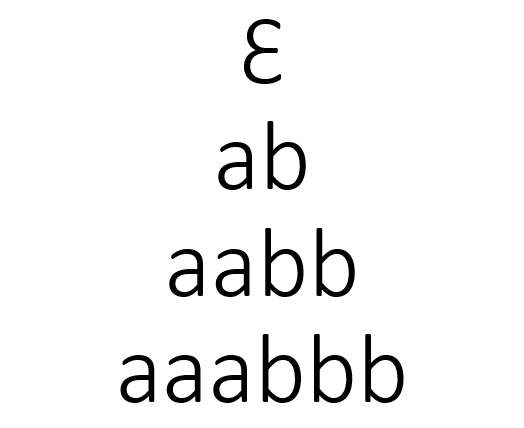
\includegraphics[scale=0.9]{Practica4/D_2.PNG}
	\end{figure}

	Con eso me percate que el número de \textbf{a} y \textbf{b} que se generan
	son iguales, y que van de 1 a n. 

	\textbf{Propuesta de solución} \\
	Después de que me percate de lo anterior, entonces pensé en crear un método
	que generara una cadena de \textbf{n} a y otra de \textbf{n} b. Y finalmente
	concatenara ambas cadenas. Dependiendo del número de cadenas que el usuario ingrese, se irán generando
	e imprimiendo.

	\newpage
	% \\\\\\\\\\\\\\\\\\\\\\\\\\\\\\\\\\\\\\\\\\\\\\\\\\\\\\\\\\\\\\\\\\\\\
	% \\\\\\\\\\\\\\\\\\\\\\\ DISEÑO DE LA SOLUCION \\\\\\\\\\\\\\\\\\\\\\\
	% \\\\\\\\\\\\\\\\\\\\\\\\\\\\\\\\\\\\\\\\\\\\\\\\\\\\\\\\\\\\\\\\\\\\\\

	\section{Diseño de la solución}
		\textbf{GRAMÁTICA}
		\begin{figure}[H]
		    \centering
		    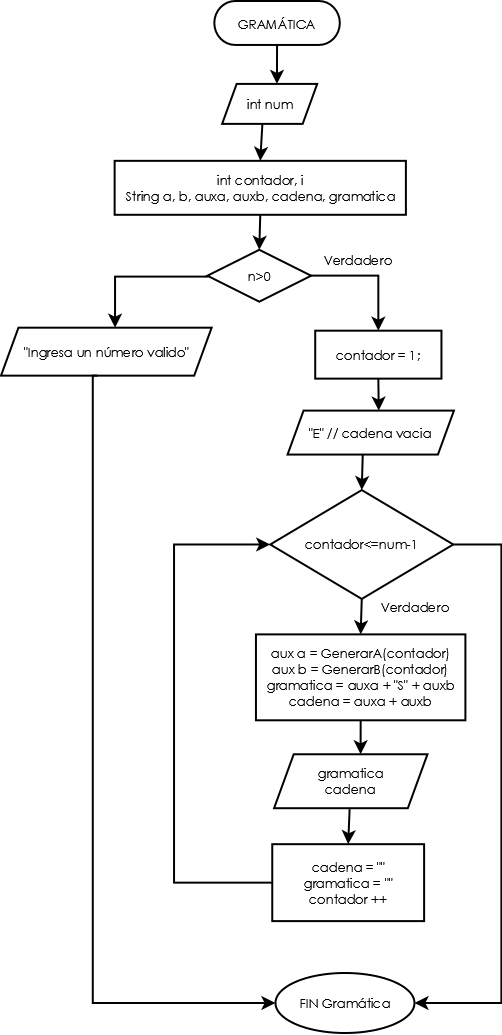
\includegraphics[scale=0.4]{Practica4/Gramatica.PNG}
		\end{figure}
		
		\textbf{GenerarA}
		\begin{figure}[H]
		    \centering
	        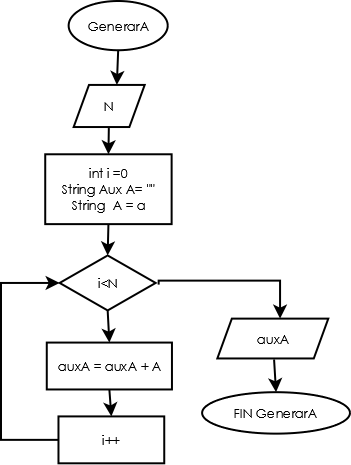
\includegraphics[scale=0.4]{Practica4/GenerarA.PNG}
		\end{figure}
		\textbf{GenerarB}
		\begin{figure}[H]
		    \centering
		    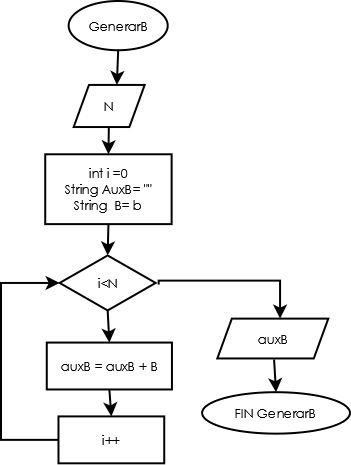
\includegraphics[scale=0.4]{Practica4/GenerarB.PNG}
		\end{figure}

	\newpage
	% \\\\\\\\\\\\\\\\\\\\\\\\\\\\\\\\\\\\\\\\\\\\\\\\\\\\\\\\\\\\\\\\\\\\\\\\\\\\\
	% \\\\\\\\\\\\\\\\\\\\\\\ IMPLEMENTACION DE LA SOLUCION \\\\\\\\\\\\\\\\\\\\\\\
	% \\\\\\\\\\\\\\\\\\\\\\\\\\\\\\\\\\\\\\\\\\\\\\\\\\\\\\\\\\\\\\\\\\\\\\\\\\\\\

	\section{Implementación de la solución}

	De forma general el programa esta estructurado de tal forma que se introduce una cadena, 
	al dar click al boton \textbf{OK} el programa empieza a validar cada uno de los estados.

	A continuación se muestra cada parte fundamental para que el programa funcione.

	\textbf{IMPLEMENTACIÓN DE GRAMÁTICA}
	\begin{lstlisting}[style=Java]
	public void Gramatica()
	{
		int num = Integer.parseInt(Cadena.getText());
		int contador, i;
		String a, b;
		String auxa, auxb, cadena, gramatica;
		a = "a"; auxa = "";
		b = "b"; auxb = "";
		if(num > 0)
		{
			contador = 1;
			AreaSalida.setText("E");
			while (contador<=num-1) // Imprime el número de cadenas que se eligen
			{
				// Se crea una cadena que contenga s a
				auxa = GenerarA(contador);
				// Se crea una cadena que contenta s b
				auxb = GenerarB(contador);
				// Cadena que muestra COMO funciona
				gramatica = auxa + "S" + auxb;
				// Cadena que muestra el resultado
				cadena = auxa + auxb;
				AreaSalida.setText(" "+AreaSalida.getText()+ "\n" + gramatica + "   " + cadena);
				cadena = ""; gramatica = "";
				contador++;
			}
		}
		else 
			AreaSalida.setText("El numero que ingresaste no es valido");
	}
	\end{lstlisting}			

	\textbf{IMPLEMENTACIÓN DE GENERAR A}
	\begin{lstlisting}[style=Java]
	public String GenerarA(int N)
	{
		int i;
		String auxA = "", A = "a";
		// Concatena el numero de a que se pidan
		for (i=0; i<N; i++)
			auxA = auxA + A;
		return auxA;
	}
	\end{lstlisting}			
	\newpage
	\textbf{IMPLEMENTACIÓN DE GENERAR B}
	\begin{lstlisting}[style=Java]
	public String GenerarB(int N)
	{
		int i;
		String auxB = "", B = "b";
		// Concatena el numero de  b que se pidan
		for (i=0; i<N; i++)
			auxB = auxB + B;
		return auxB;
	}

	\end{lstlisting}			
\newpage

	% \\\\\\\\\\\\\\\\\\\\\\\\\\\\\\\\\\\\\\\\\\\\\\\\\\\\\\\\\\\\\\
	% \\\\\\\\\\\\\\\\\\\\\\\ FUNCIONAMIENTO \\\\\\\\\\\\\\\\\\\\\\\
	% \\\\\\\\\\\\\\\\\\\\\\\\\\\\\\\\\\\\\\\\\\\\\\\\\\\\\\\\\\\\\\

	\section{Funcionamiento}
	Primero que nada, mostramos la interfaz inicial. Observamos que el 
	usuario tiene la oportunidad de ingresar el número de cadenas que 
	desea que se muestren. Al dar click en el botón OK, se mostrarán 
	las cadenas generadas.

	La pantalla inicial es la siguiente:
	
	\begin{figure}[H]
	        \centering
	        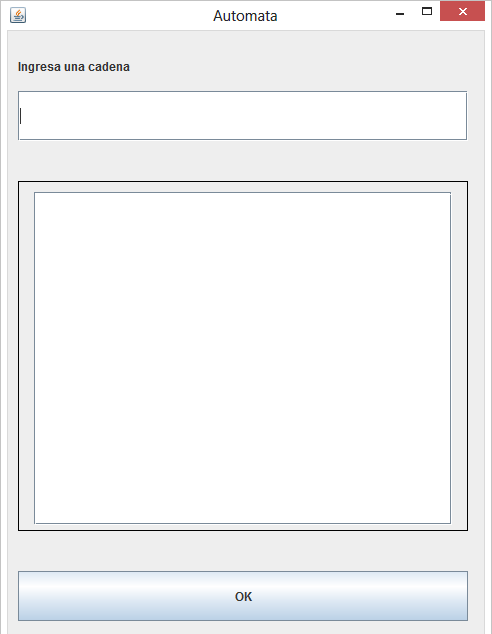
\includegraphics[scale=0.9]{Practica4/F_1.PNG}
	\end{figure}
	
	\begin{figure}[H]
	        \centering
	        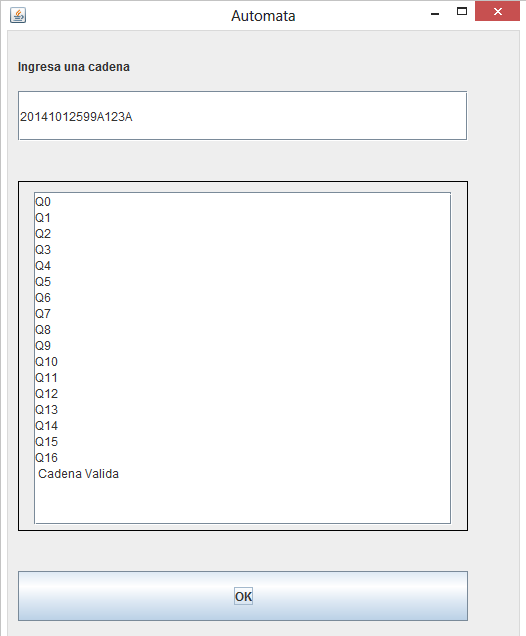
\includegraphics[scale=0.9]{Practica4/F_2.PNG}
	\end{figure}
	
	\begin{figure}[H]
	        \centering
	        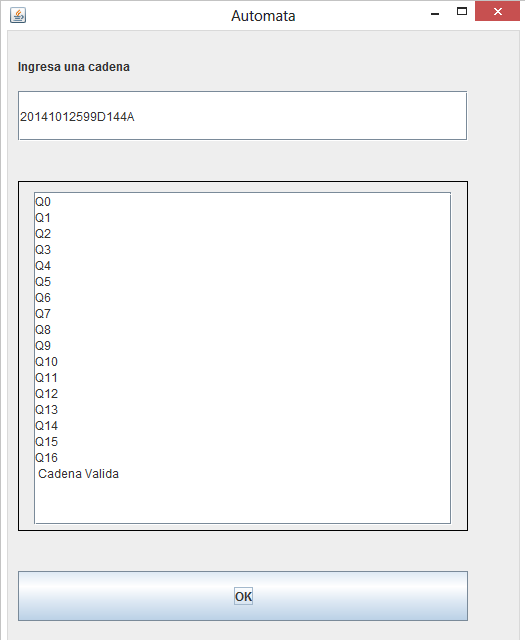
\includegraphics[scale=0.9]{Practica4/F_3.PNG}
	\end{figure}

	\begin{figure}[H]
	        \centering
	        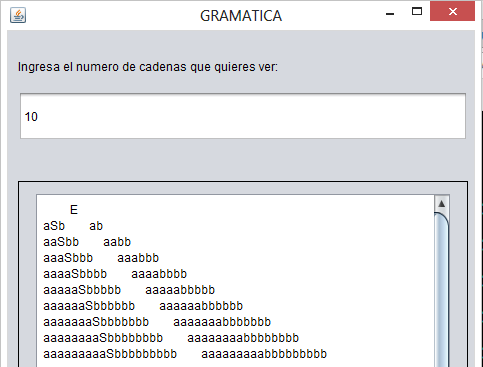
\includegraphics[scale=0.9]{Practica4/F_4.PNG}
	\end{figure}


	% \\\\\\\\\\\\\\\\\\\\\\\\\\\\\\\\\\\\\\\\\\\\\\\\\\\\\\\\\\\\
	% \\\\\\\\\\\\\\\\\\\\\\\ CONCLUSIONES \\\\\\\\\\\\\\\\\\\\\\\
	% \\\\\\\\\\\\\\\\\\\\\\\\\\\\\\\\\\\\\\\\\\\\\\\\\\\\\\\\\\\\
	\section{Conclusiones}

	Al terminar está práctica pude ver que las gramáticas libres
	de contexto te permiten generar cadenas de forma recursiva y 
	de cierta forma más sencilla que las anteriores, puesto que 
	es muy recursivo.

	Además que me parece muy interesante que sean utilizadas para
	validar las sentencias en los lenguajes de programación.

	% \\\\\\\\\\\\\\\\\\\\\\\\\\\\\\\\\\\\\\\\\\\\\\\\\\\\\\\\\\\\
	% \\\\\\\\\\\\\\\\\\\\\\\ BIBLIOGRAFIA \\\\\\\\\\\\\\\\\\\\\\\
	% \\\\\\\\\\\\\\\\\\\\\\\\\\\\\\\\\\\\\\\\\\\\\\\\\\\\\\\\\\\\

	 \nocite{ref1, ref2}
	\bibliography{referencias}
\end{document}